\documentclass[12pt,a4paper]{article}
\usepackage{amsmath}
\usepackage{amssymb}
\usepackage{geometry}
\usepackage{enumerate}
\usepackage{graphicx}
\usepackage{subfigure}
\usepackage{ctex}
\usepackage{float}
\usepackage{makecell}
\usepackage{float}
\usepackage{multirow}
%-----------------------------------%
% 宏包定义enumerical间距
\usepackage{paralist} 
\let\itemize\compactitem 
\let\enditemize\endcompactitem 
\let\enumerate\compactenum 
\let\endenumerate\endcompactenum 
\let\description\compactdesc 
\let\enddescription\endcompactdesc
%------------------------------------
\newcommand{\tabincell}[2]{\begin{tabular}{@{}#1@{}}#2\end{tabular}}
%------------------------------------
\begin{document}
\section{Introduction}
\subsection{Objectives}
  The objective of this experiment is to study the characteristics of an Op Amp, we learn to build circuit with the LM 741 Op Amp to make an non-inverting and inverting amplifiers with fixed gain.
\subsection{Apparatus and Theoretical Background}
An Op Amp is an integrated circuit which has two terminals for input signals: inverting (labled -) and non-inverting (labeled +), a terminal for the output signal, two terminals for the power supply voltages: positive +$V_{CC}$ and negative -$V_{CC}$. In this lab, we use the LM 471 Op Amp which has 8 pins but only 5 of them are used in this lab. The function of each pin is labled on the following figure 1.
%---------------------------------
  \begin{figure}[H]
  \centering
  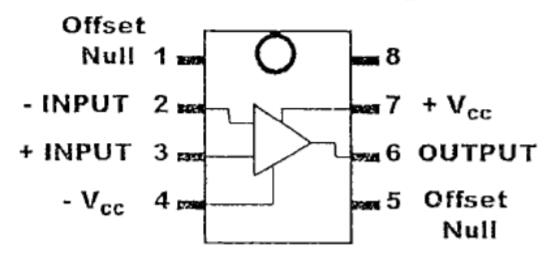
\includegraphics[width=.6\textwidth]{Figure1.jpg}
  \caption{Pin numbers for LM 741 Op Amp}
  \label{img} 
\end{figure}
%--------------------------------- 

The gain of amplifier circuit is defined as 
$$\textit{Voltage Gain} = \frac{\textit{Output Voltage}}{\textit{Input Voltage}}$$

The circuit for the inverting Op Amp is shown in the following figure 2. The inverting Op Amp have the gain
$$Gain = \frac{V_{output}}{V_s}= -\frac{R_F}{R_A}$$
%---------------------------------
  \begin{figure}[H]
  \centering
  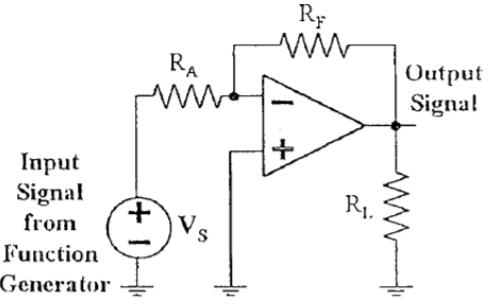
\includegraphics[width=.6\textwidth]{Figure2.jpg}
  \caption{Inverting Op Amp}
  \label{img} 
\end{figure}
%--------------------------------- 

The circuit for the non-inverting Op Amp is shown in the following figure 3. The non-inverting Op Amp have the gain
$$Gain = \frac{V_{output}}{V_s}= 1+\frac{R_F}{R_A}$$
%---------------------------------
  \begin{figure}[H]
  \centering
  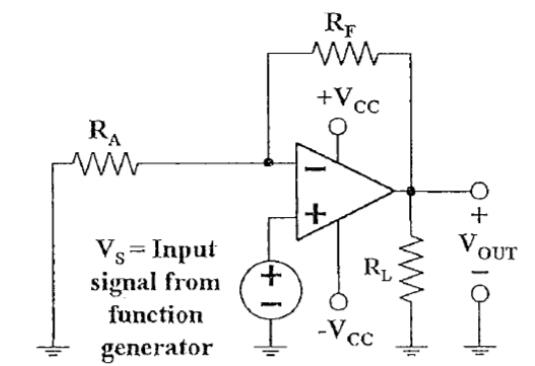
\includegraphics[width=.6\textwidth]{Figure3.jpg}
  \caption{non-inverting Op Amp}
  \label{img} 
\end{figure}
%--------------------------------- 

In this lab, there are two important equipments called \textbf{Function generator} and \textbf{Oscilloscope}.
We can change the amplitude, frequency of wave using function generator.
%---------------------------------
  \begin{figure}[H]
  \centering
  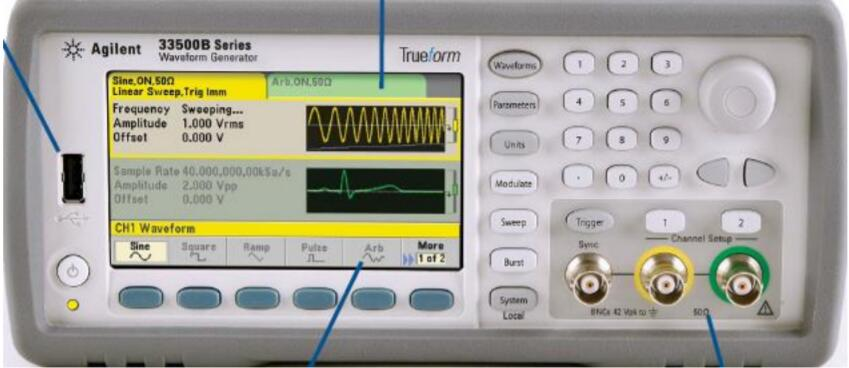
\includegraphics[width=.6\textwidth]{Figure4.jpg}
  \caption{Function generator}
  \label{img} 
\end{figure}
%--------------------------------- 
The oscilloscope is used to observe the output voltage. We use "Auto scale" to achieve an output on the screen with proper scale automatically, use "Meas" to measure the wave, use "1/2" to show or hide the wave we detecting through channel 1/2.
%---------------------------------
  \begin{figure}[H]
  \centering
  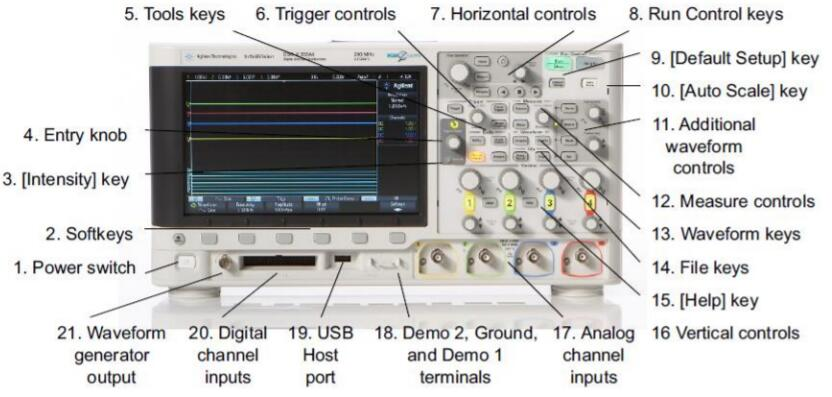
\includegraphics[width=.6\textwidth]{Figure5.jpg}
  \caption{Oscilloscope}
  \label{img} 
\end{figure}
%--------------------------------- 
\subsection{Measurement}
\subsubsection{Non-inverting amplifier}
We build the circuit shown in the following figure whose $R_F$ = 100$\Omega $, $R_A = 50\Omega $. We use the function generator to generate an sine wave and use it as the input voltage. We set the initial amplitude of the sine wave to 0.1$V_{PP}$ then use the oscilloscope to measure the output voltage. Later, we increase the input voltage 0.1$V_{PP}$ at a time and record the corresponding output until the output voltage is saturated.
%---------------------------------
  \begin{figure}[H]
  \centering
  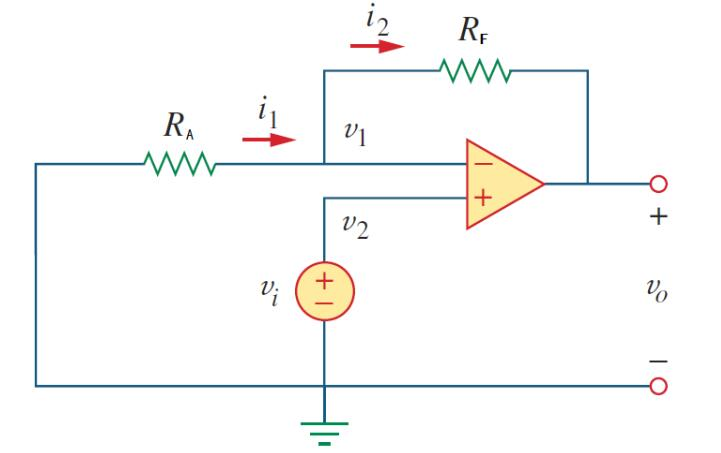
\includegraphics[width=.6\textwidth]{Figure6.jpg}
  \caption{Circuit for non-inverting amplifier}
  \label{img} 
\end{figure}
%--------------------------------- 
\subsubsection{Inveritng amplifier}
We build the circuit shown in the following figure, while still use the same $R_F$ and $R_A$. Similarly, we do the same operation and measurement.
%---------------------------------
  \begin{figure}[H]
  \centering
  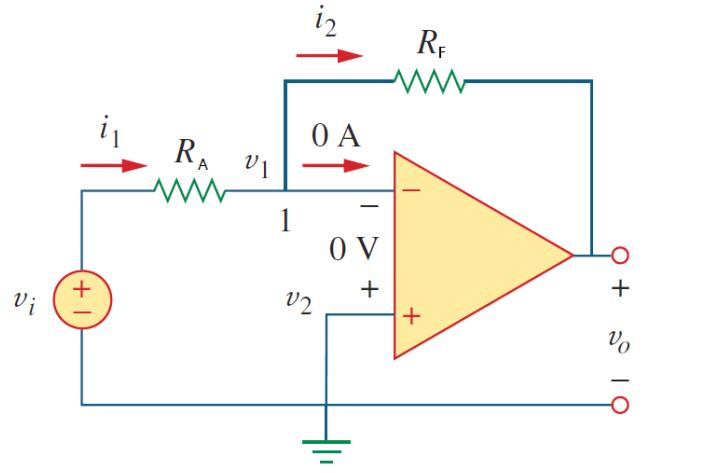
\includegraphics[width=.6\textwidth]{Figure7.jpg}
  \caption{Inverting amplifier}
  \label{img} 
\end{figure}
%--------------------------------- 
\section{Results and Discussion}
Before building the circuit of non-inverting and inverting amplifiers, we first measure the resistance of the two resistors we use.
%--------------------------------- 
\begin{table}[htp]
\centering
\begin{tabular}{|c|c|}
\hline
$R_1[\Omega ]$ & 50.2  \\ \hline
$R_f[\Omega ]$ & 101.0 \\ \hline
\end{tabular}
\caption{The resistance of the resistors}
\end{table}
%---------------------------------
According to the measurement, we expect that the $$\frac{R_f}{R_1} = \frac{50.2}{101.0} = 2.012$$
%---------------------------------
Then we measure the voltage supplied to the op amp.
%---------------------------------
\begin{table}[htp]
\centering
\begin{tabular}{|c|c|}
\hline
+$V_{CC}$ & 5  \\ \hline
+$V_{CC}$ & -5 \\ \hline
\end{tabular}
\caption{The voltage supplied to the op amp}
\end{table}
%---------------------------------
\subsection{Non-inverting Amplifier}
After that, we build the circuit of non-inverting amplifier and measured the input/output relationship.
%---------------------------------
\begin{table}[htp]
\centering
\begin{tabular}{|c|c|}
\hline
$V_{PP(in)}${[}V{]} & $V_{PP(out)}${[}V{]} \\ \hline
0.10                & 0.36                 \\ \hline
0.20                & 0.66                 \\ \hline
0.30                & 0.96                 \\ \hline
0.40                & 1.25                 \\ \hline
0.50                & 1.55                 \\ \hline
0.60                & 1.82                 \\ \hline
0.70                & 1.82                 \\ \hline
0.80                & 1.82                 \\ \hline
0.90                & 1.83                 \\ \hline
1.00                & 1.83                 \\ \hline
\end{tabular}
\caption{the input/output relation of the non-invering op amp}
\end{table}
%---------------------------------

Then, we plot the relationship of input and output. The linear fit is shown in the following figure.
%---------------------------------
  \begin{figure}[H]
  \centering
  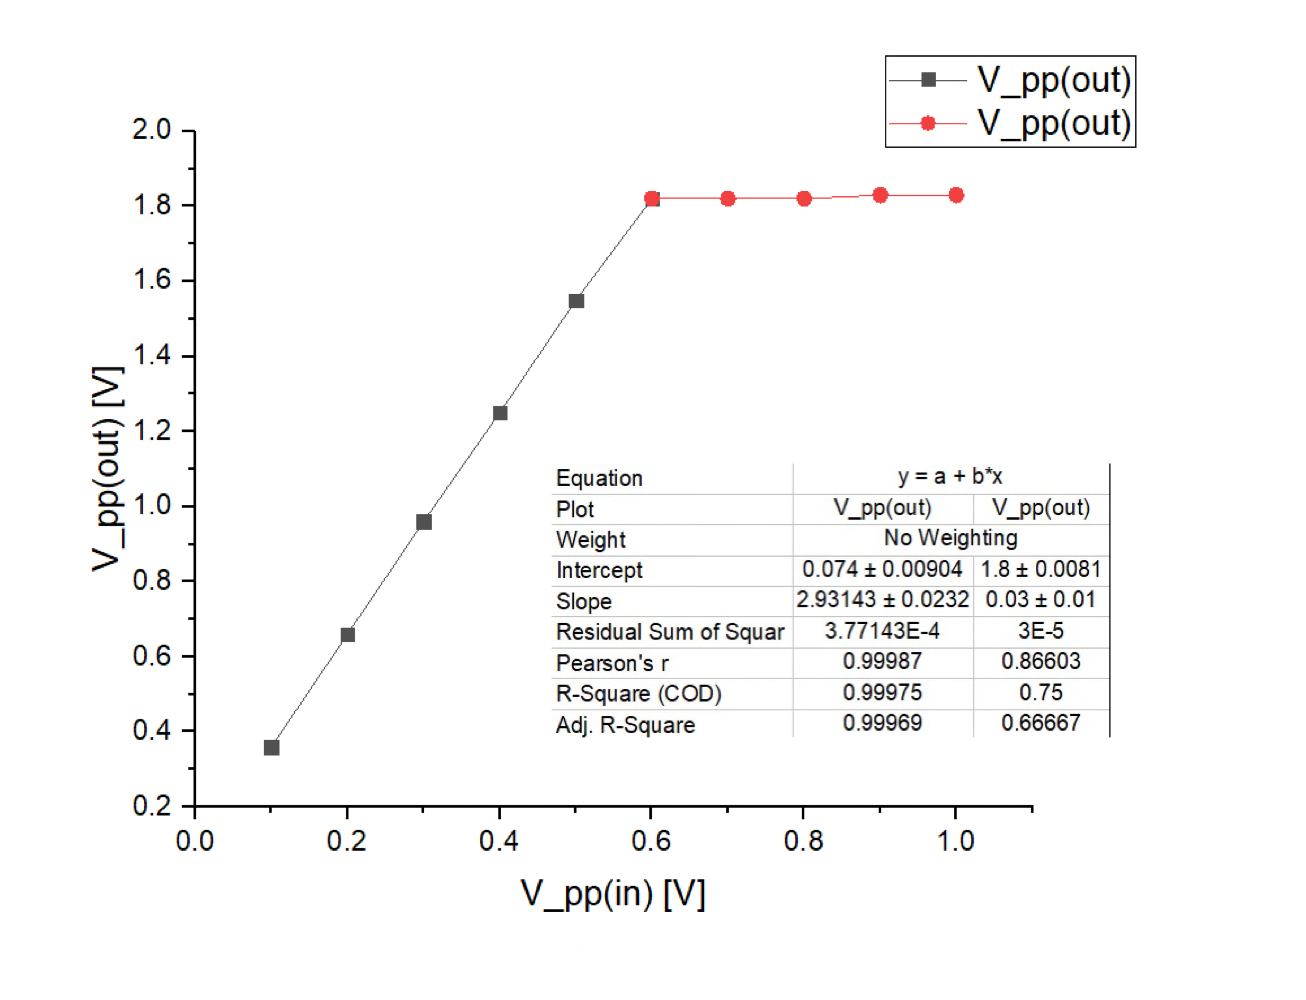
\includegraphics[width=.8\textwidth]{Figure8.png}
  \caption{the input/output relation of the non-invering op amp}
  \label{img} 
\end{figure}
%--------------------------------- 

From the figure we see that when the $V_{in} <= 0.6V$ the amplifier works linearly in this region.
The gain shown in the linear fit is 2.93, the theoritical value of the gain is 
$$Gain = 1+\frac{R_{f}}{R_1} = 1+2.012 = 3.012$$

The relative error is $$error = 1- \frac{2.93}{3.012}\times 100\% = 2.7\%$$
Therefore, the actual gain is very close to the theoritical value.
 The Adj. R-Square is 0.99969 which indicate the amplifier works well and meet our expectation. According to the linear fit, we find that the saturation voltage of this op amp is 1.8V. However, the theoretical value is $V_{CC}$ which is 5V. This will be discussed in the Conclusion part later.


\subsection{Inverting Amplifier}
In this part of the experiment, we intend to study the characteristics of the input/output relationship of the inverting amplifier. We use the same voltage source and the same resistors. The only difference lies in the way we connect the circuit to make it an inverting amplifier.

The original data is shown in the following table.
\begin{table}[htp]
\centering
\begin{tabular}{|c|c|}
\hline
$V_{PP(in)}${[}V{]} & $V_{PP(out)}${[}V{]} \\ \hline
0.10                & -0.23                \\ \hline
0.20                & -0.43                \\ \hline
0.30                & -0.63                \\ \hline
0.40                & -0.83                \\ \hline
0.50                & -1.01                \\ \hline
0.60                & -1.21                \\ \hline
0.70                & -1.41                \\ \hline
0.80                & -1.60                \\ \hline
0.90                & -1.78                \\ \hline
1.00                & -1.97                \\ \hline
\end{tabular}
\caption{the input/output relation of the invering op amp}
\end{table} 

%---------------------------------
  \begin{figure}[H]
  \centering
  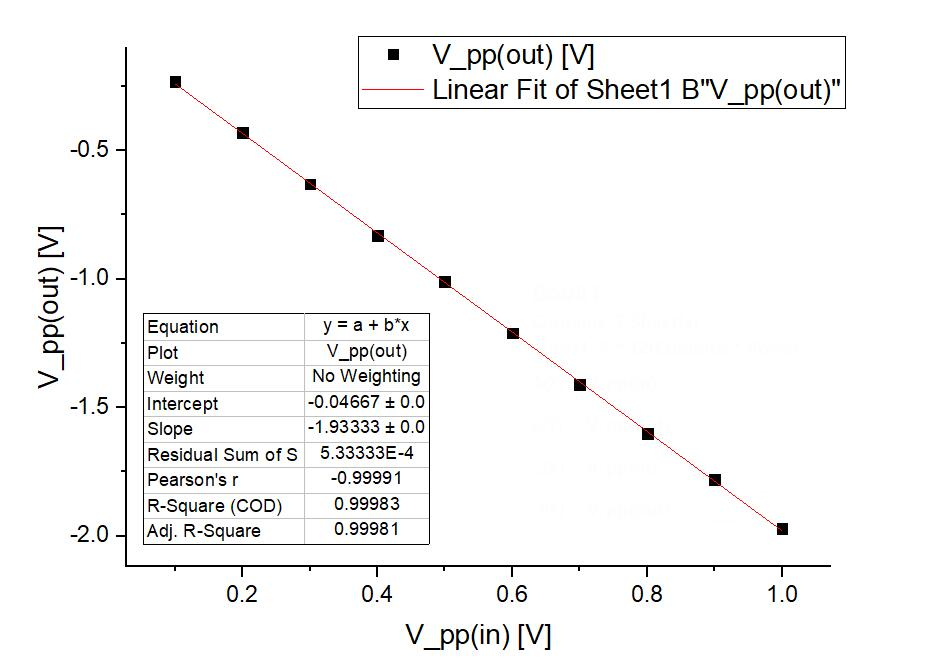
\includegraphics[width=.8\textwidth]{Figure9.jpg}
  \caption{the input/output relation of the invering op amp}
  \label{img} 
\end{figure}
%--------------------------------- 

From the linear fit we find that the relationship between input and output is linear which meet our expectation. According to the linear fit, the gain which is the slope is -1.933. The theoritical value of gain is calculated as
$$Gain = -\frac{R_f}{R_1}= -2.012$$
Comparing to the exact value, the relative error is 
$$Error = 1- \frac{-1.933}{-2.012} = 3.93\%$$
This relative error is small and as shown in the linear fit, the Adj.R-Square is 0.99981 which indicate the linear relationship between the input voltage and output voltage is clear.
\section{Conclusion}
In this experiment, we use different cuircuit to make an non-inverting amplifier and inverting one. We measured the output voltage and plot the relationship between its input and output. We find that before the saturation voltage is reached, the amplifier works linearly. 

However, we have met some problems in this lab. During the lab, we find that many things will go wrong due to the unstability of the circuit elements. When we fail to get the correct result, there's maybe something wrong with some elements thus take various time to fix it.

Also, in the non-inverting amplifier's part, we find that the saturation voltage is only 1.8V. While the theoretical value is the $V_{CC}$ which is 5V. So I seach on the internet and find this maybe caused by op amp's saturation voltage drop. It means due to some design and property of the op amp's material, the amplifier cannot meet exactly $V_{CC}$, instead, it the saturation voltage maybe lower than the theorital value.


\end{document}